% !TeX root = document.tex
% !TeX encoding = UTF-8 Unicode

\subsection{Results}%
\label{subsec:fo-results}

\begin{slide}{Results (Puma 560)}
  \begin{columns}[c]
    \begin{column}{0.55\textwidth}
      \begin{figure}[ht!]
        \centering
        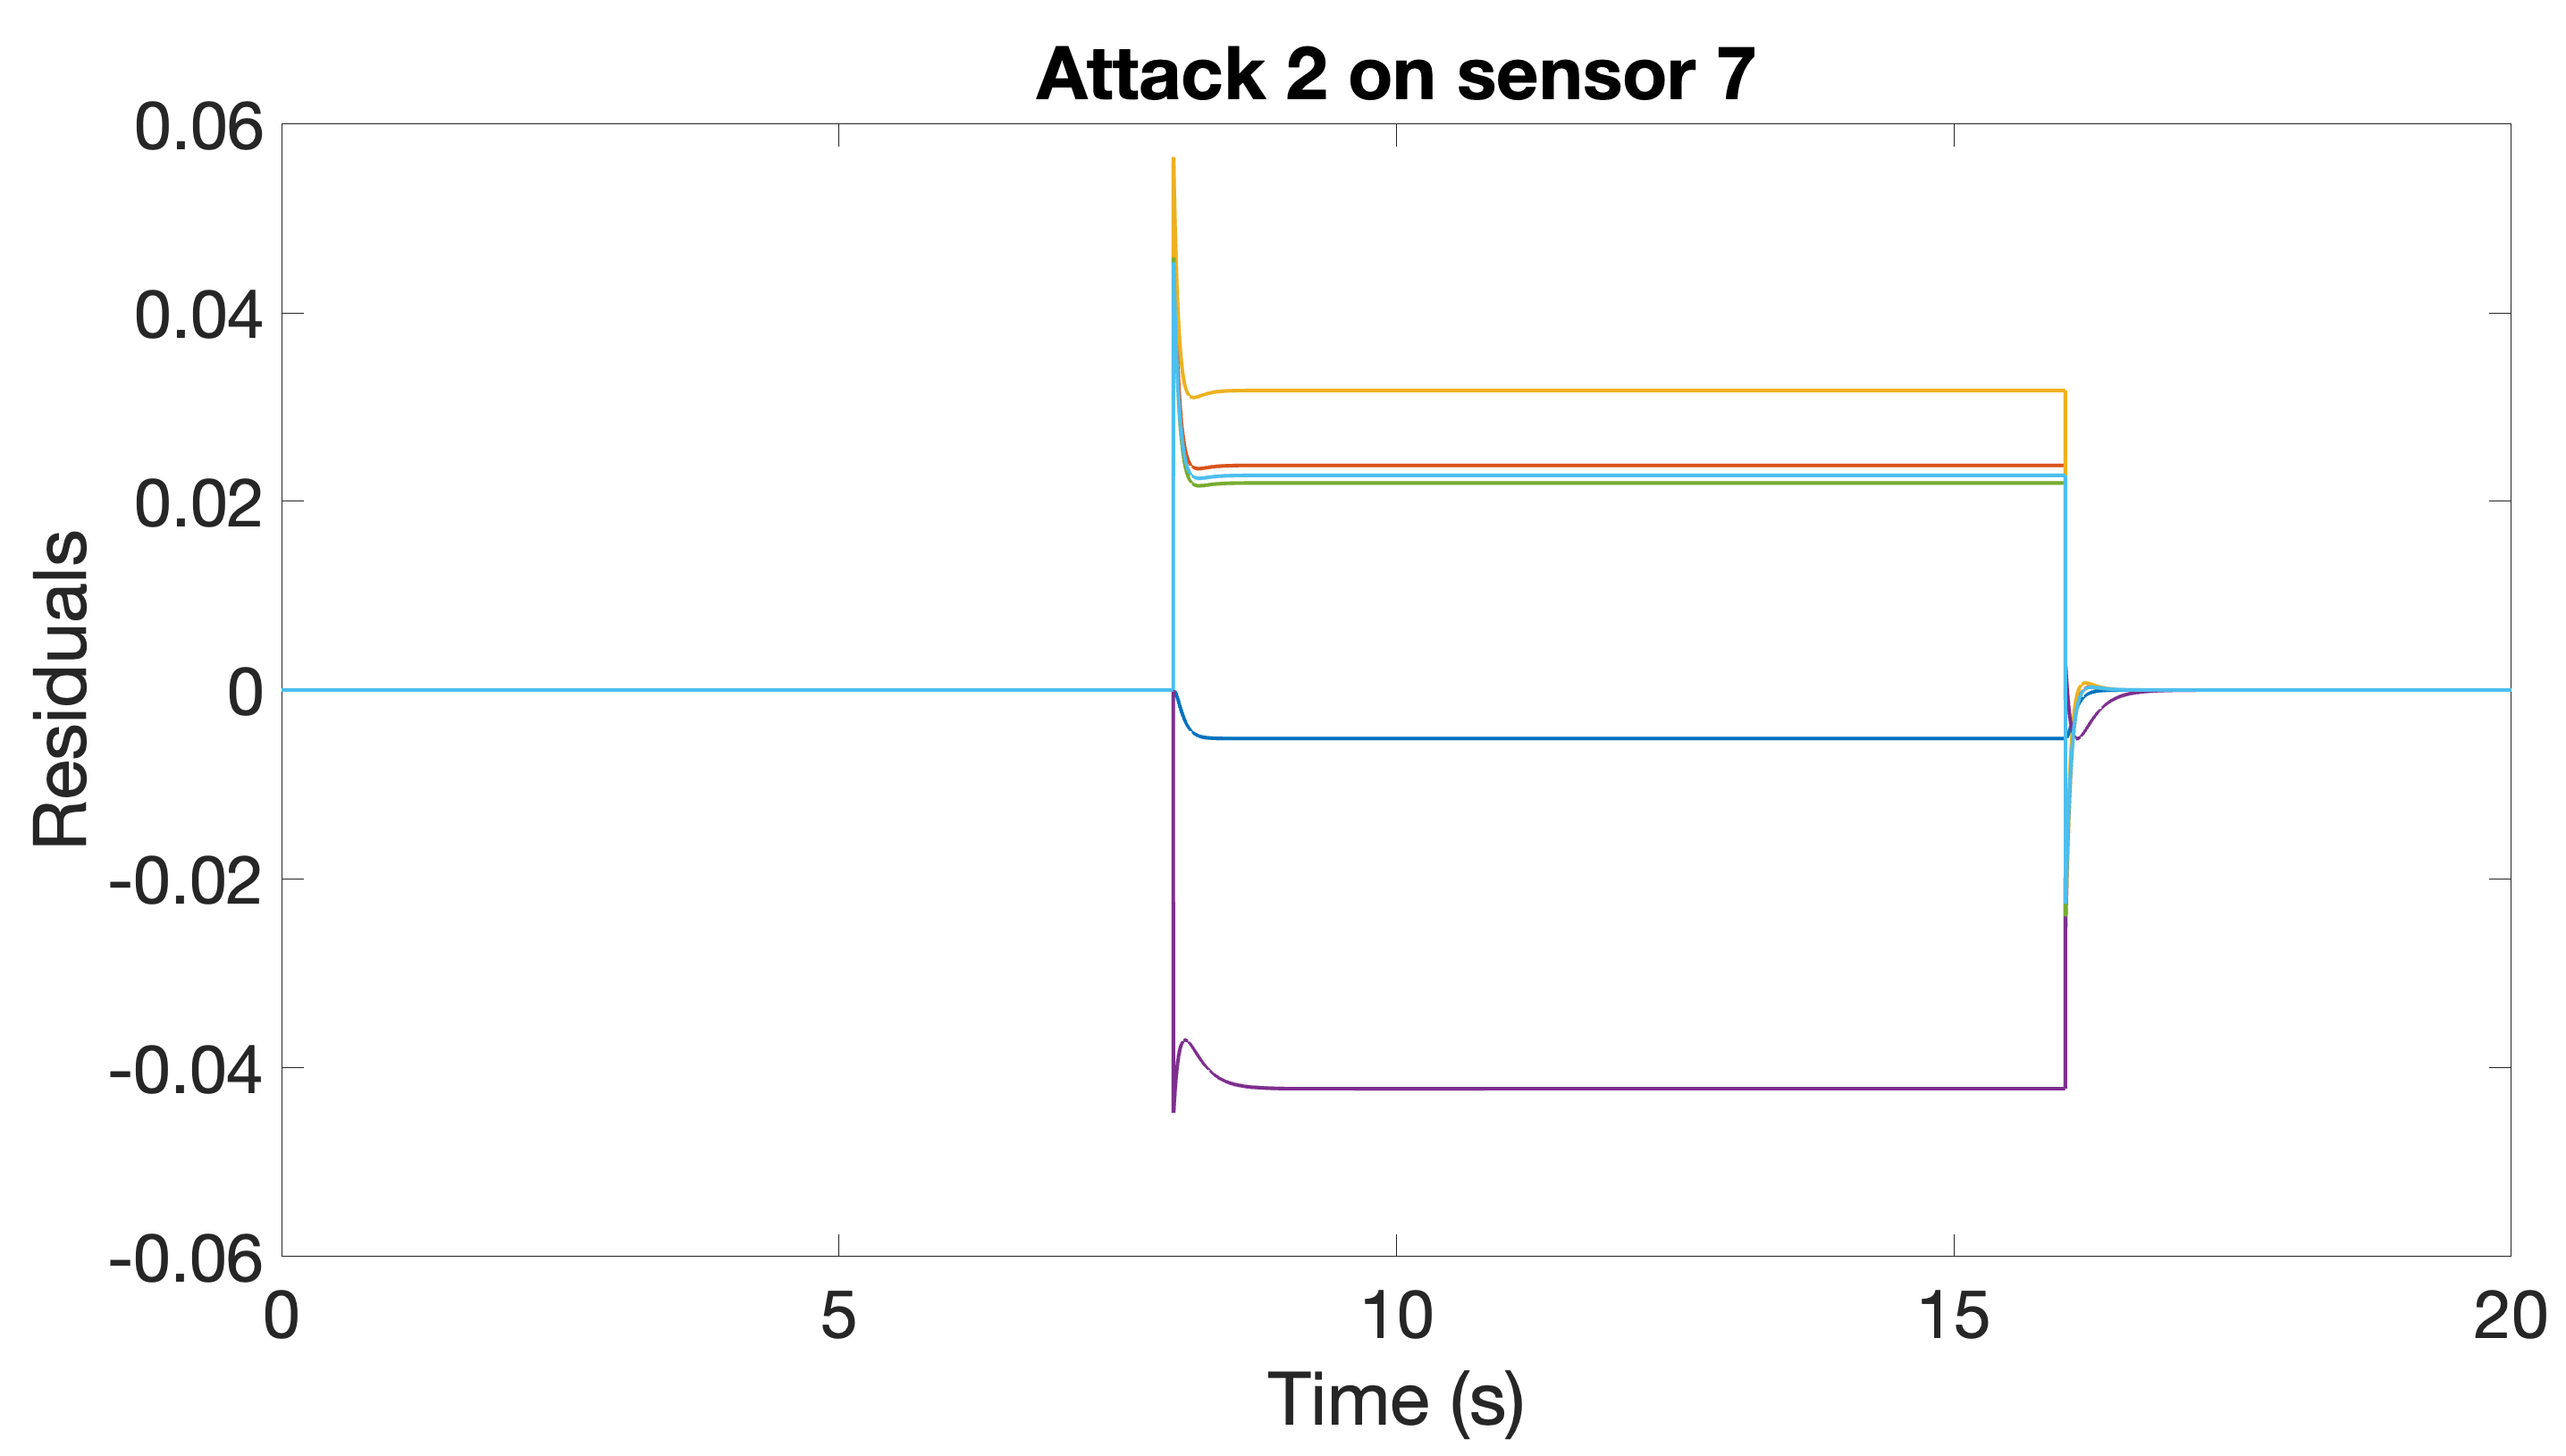
\includegraphics[width=0.9\linewidth]{s7a2}
        \caption{Residuals for attack on sensor 7, with \(\delta=1\)}%
        \label{fig:s7a2}
      \end{figure}
    \end{column}%
    \hfill%
    \begin{column}{0.55\textwidth}
      \begin{figure}[ht!]
        \centering
        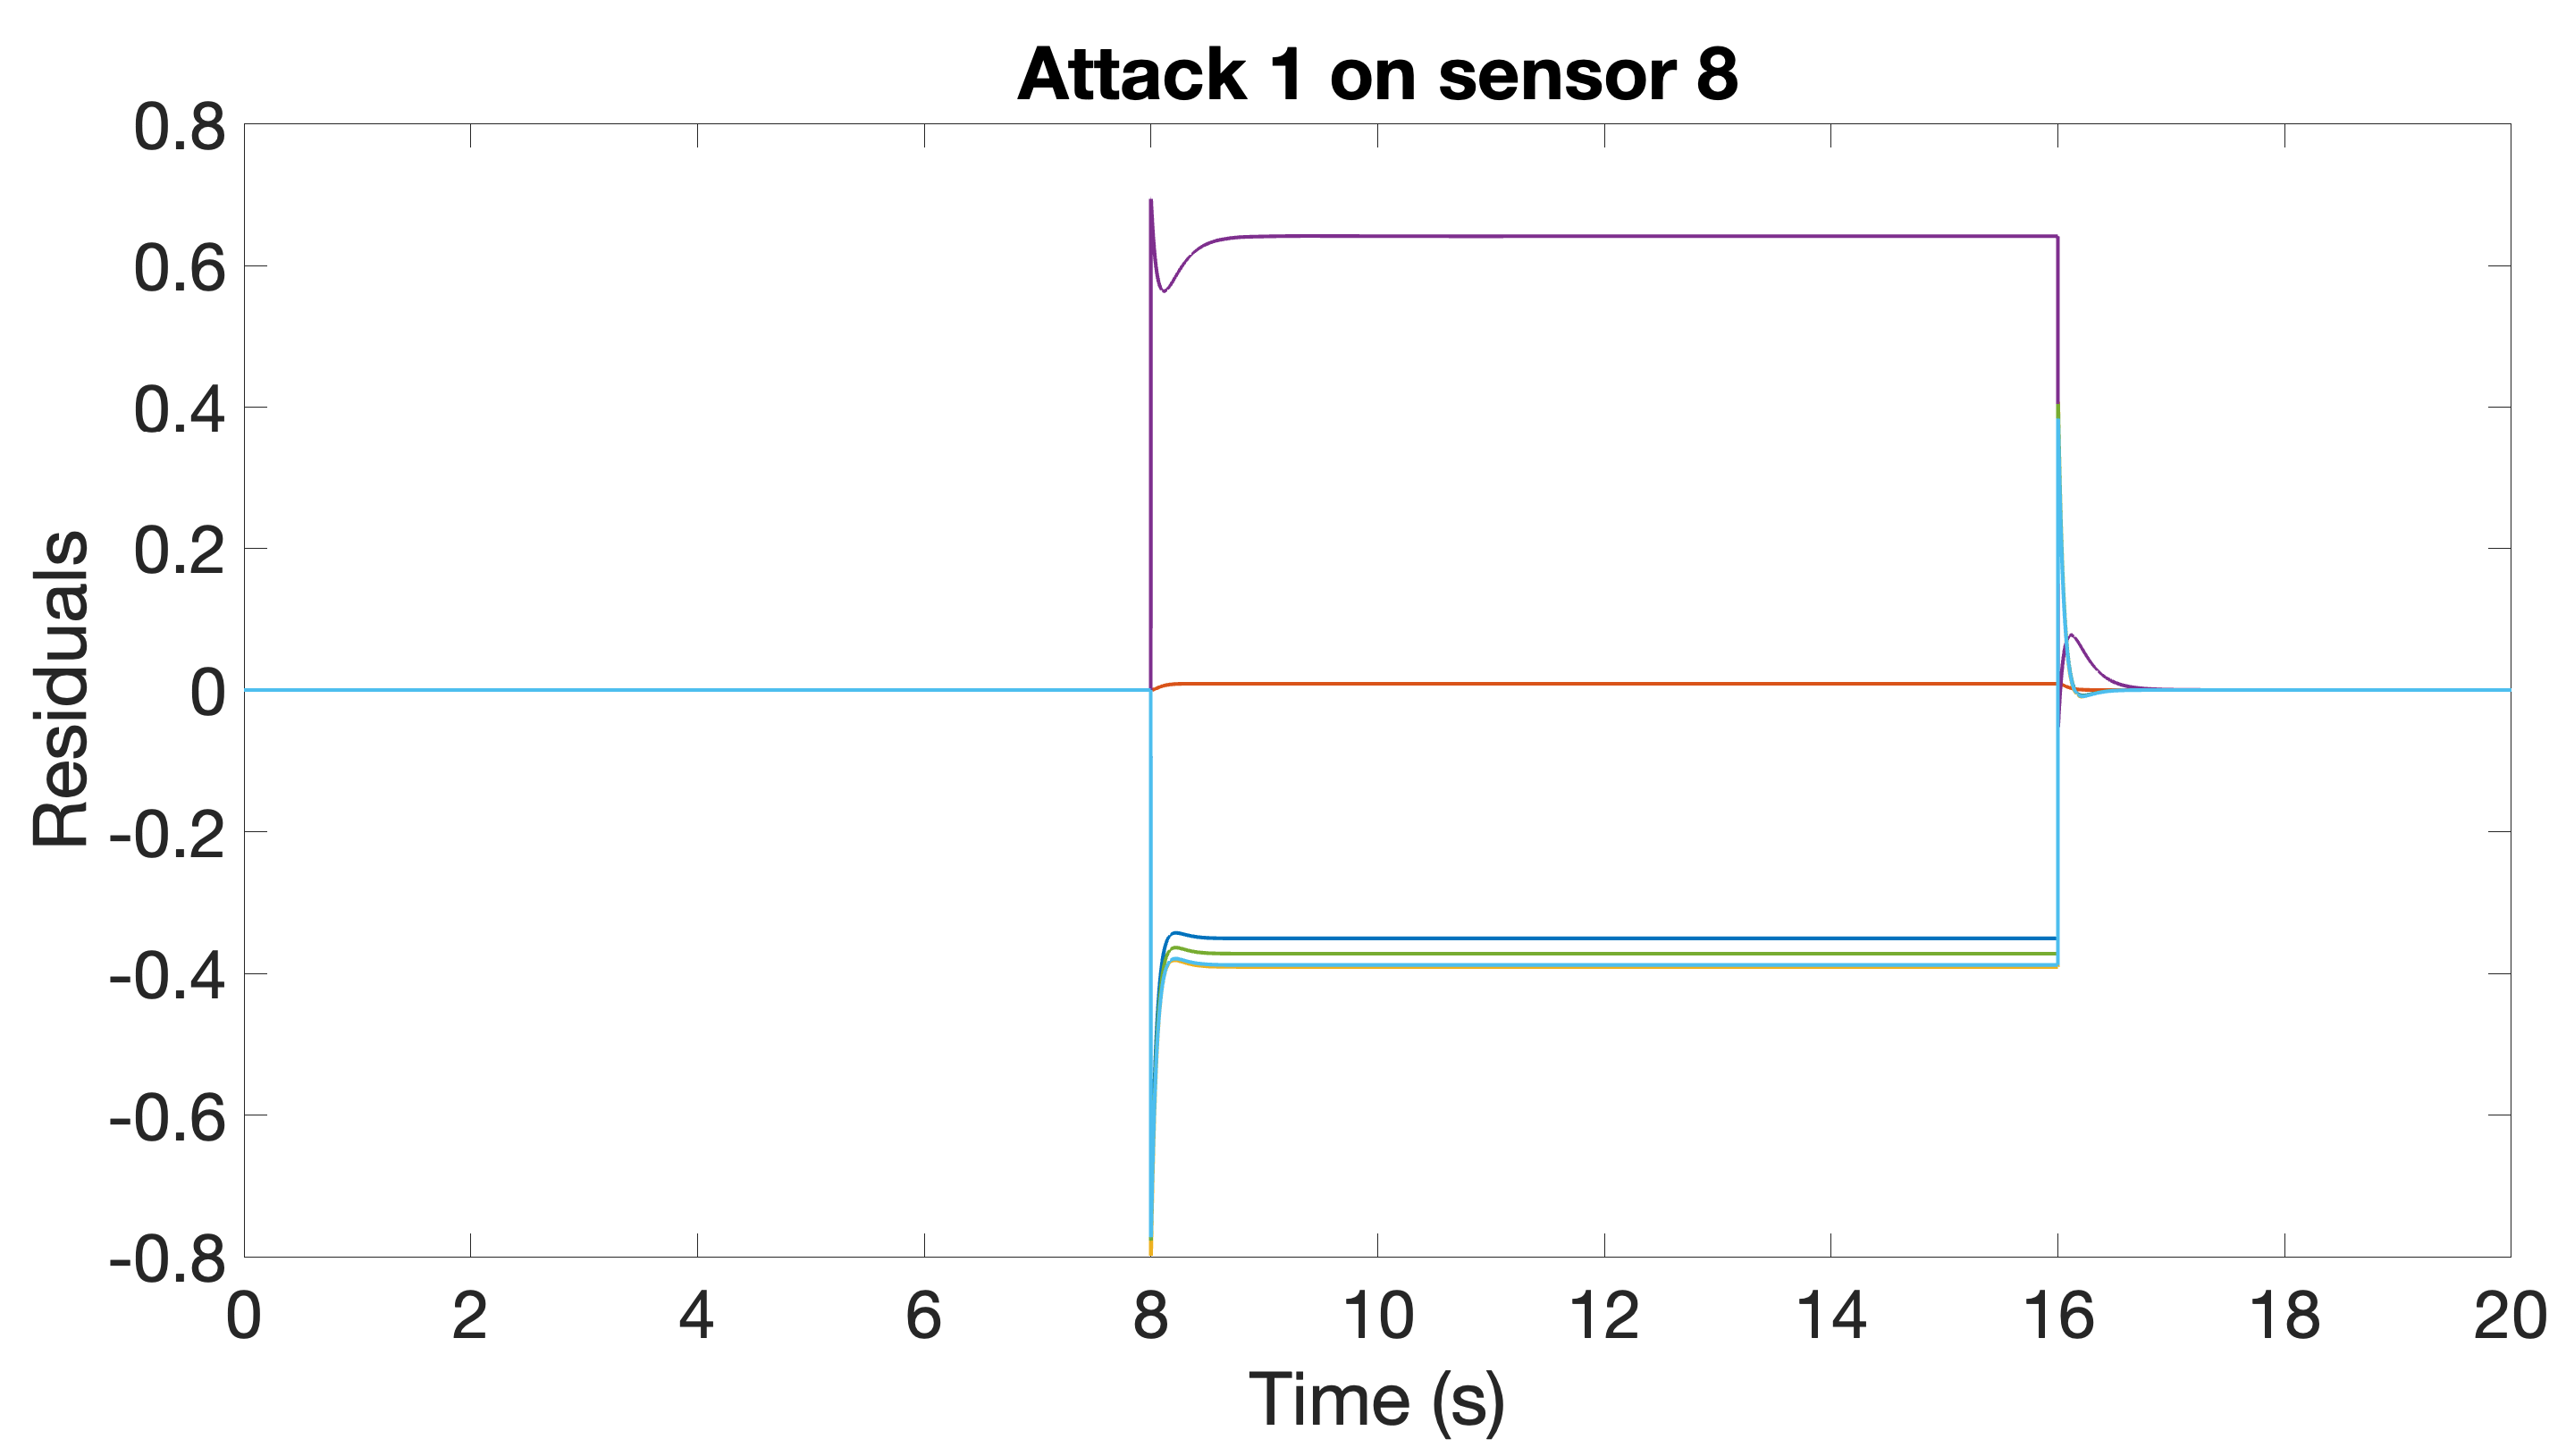
\includegraphics[width=0.9\linewidth]{s8a1}
        \caption{Residuals for attack on sensor 8, copying the values from
          sensor 9}%
        \label{fig:s8a1}
      \end{figure}
    \end{column}%
  \end{columns}
\end{slide}

\begin{slide}{Results (IEEE118)}
  Functional Observer with 120 states.
  \begin{columns}[c]
    \begin{column}{0.55\textwidth}
      \begin{figure}[ht!]
        \centering
        \includegraphics[width=0.9\linewidth]{s117a3}
        \caption{Residuals for multiplicative attack on state 117}%
        \label{fig:s117a3}
      \end{figure}
    \end{column}%
    \hfill%
    \begin{column}{0.55\textwidth}
      \begin{figure}[ht!]
        \centering
        \includegraphics[width=0.9\linewidth]{s155a1}
        \caption{Residuals for state-copy attack on state 155}%
        \label{fig:s155a1}
      \end{figure}
    \end{column}%
  \end{columns}
\end{slide}
